\documentclass[a4paper,10pt]{report}
\usepackage[utf8]{inputenc}
\usepackage{gensymb}
\usepackage{textcomp}
\usepackage{graphicx}

% Title Page
\title {\strong{Week 1 Update}}
\author{Rajat Saxena}

\begin{document}
\maketitle

\section{Kinect Skeleton Tracking}

\subsection{Introduction}
\begin{itemize}
 \item In skeleton tracking, a human body is represented by 17 joints (Head, Neck, Torso, Left and Right Collar, L/R Shoulder, L/R Elbow, L/R Wrist, L/R Hip, L/R Knee and L/R Foot) along with the tracking confidence.
 \item Each joint is represented by its 3d coordinates.
 \item Kinect uses per pixel, body part recognition as an intermediate step to track skeleton. Evaluating each pixel separately avoids a combinatorial search over the different body joints.
\end{itemize}

\newline
\newline
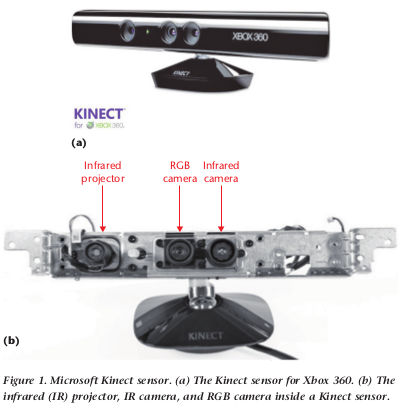
\includegraphics[scale=0.4,keepaspectratio=true]{./3.png}
% 3.png: 0x0 pixel, 0dpi, nanxnan cm, bb=

\newline
\newline
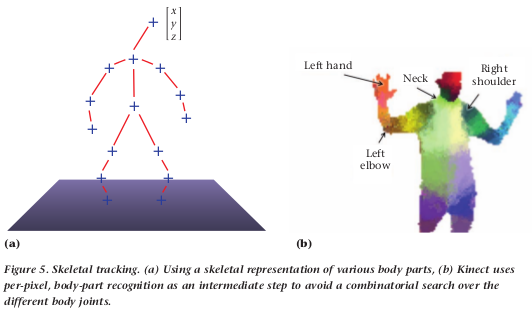
\includegraphics[scale=0.4]{./4.png}
% 4.png: 0x0 pixel, 0dpi, 0.00x0.00 cm, bb=
\newline
\newline

\section{Microsoft SDK - Skeleton Tracker}

\subsection{Introduction}
The Microsoft Kinect provides a convenient and inexpensive depth sensor and with the SDK, a skeleton tracker. This doc covers the evalaution of noise, accuracy, resolution and latency of the skeleton tracking software.

\subsection{Range of Kinect}
Experiments were conducted to find out how far and close user can be from the imaging sensor in order to be track skeleton. Below are the results:
\begin{itemize}
 \item The angular range of the device is 57\textdegree x 43\textdegree (horizontal x vertical)
 \item This can be extended vertically by using the software controls for tilt motor, this has a range of 54\textdegree
 \item Microsoft recommends an optimal range of 1.2-3.5m from the sensor. But after testing on the system, results indicated that a skeleton could be acquired within a range of 0.85-4m from the camera.
\end{itemize}

\subsection{Noise}
Tracker noise causes the rendered image to jitter on screen. 1000 samples of the central position for a tracked skeleton standing 2.0m from the sensor were taken and mean position and standard deviation were calculated.\newline
Results:
\begin{itemize}
 \item 3D noise was found be 1.3m with a sd=0.75mm at 1.2m
 \item 3D noise at 3.5m was 6.9mm and sd=5.6mm
 \item Noise differed by dimension: x averaged 4.1mm, y 6.2mm, and z 8.1mm.
\end{itemize}

\subsection{Accuracy}
Focus on relative accuracy was more rather than absolute accuracy. To test, a straight wooden meter stick positioned 2m from the sensor was taken as reference which was running approximately along the x axis. A marker was affixed to a user’s wrist to give a consistent position relative to the physical skeleton and the marker was placed along the meter stick. 25 samples were taken per point to reduce the effects of noise and measured distances between 100mm and 500mm. \newline
Results are as follows:
\begin{itemize}
 \item The average error in the tests was 5.6mm, with a sd=8.1mm
 \item To test scaling of accuracy with additional users in view, a long metal bar was used, 250mm segments, and a tape measure for reference. Error grew from 1.4mm with one user to 1.8mm with two users to 2.4mm with three users.
 \item No differences were found with respect to dimensions, including dpeth even after multiple tests.
\end{itemize}

\subsection{Latency}
Latency was measured using USB mouse relatively. Minimum latency from windows( system used to test) comes to be around 20ms. A test was conducted with two skeletons using a simple pendulum (a hand moving shoulder-to-shoulder). \newline
Results are as follows:
\begin{itemize}
\item When the program was running at its normal frame rate of 30 Hz, the relative latency was found to be 106 ms on average, with a standard deviation of 23 ms and a maximum of 156 ms. 
\item When the program was running more slowly, the relative latency was found to average 202 ms, with a standard deviation of 26 ms and a maximum of 270 ms. 
\item With a single skeleton to track, the program generally maintained a 30 Hz update rate, but it would on occasion drop. 
\item With two or three users, the frame rate was generally between 18-20 Hz.
 \item with one skeleton, mean latency= 146ms (max=243ms)
 \item with two skeleton, mean latency = 234ms (max=386ms) 
 \item with three skeleton, mean latency = 205ms (max=490ms)
\end{itemize}

\subsection{Resolution}
To establish resolution, error values less than the accuracy measurements with standard deviation less than the noise measurement were taken. This was done separately for depth(z) and one lateral dimension(x). Measurement were taken 2m from the sensor using the protocol of relative accuracy test, with distances of 1-5mm.\newline
Results:
\begin{itemize}
 \item Lateral resolution was found to be 3mm (0.086\textdegree), in agreement with PrimeSense, makers of the depth sensor. 
 \item Also measured depth resolution, 2mm, was much better than the specification of 10mm because of interpolation of joints data.
\end{itemize}

\newline
\newline
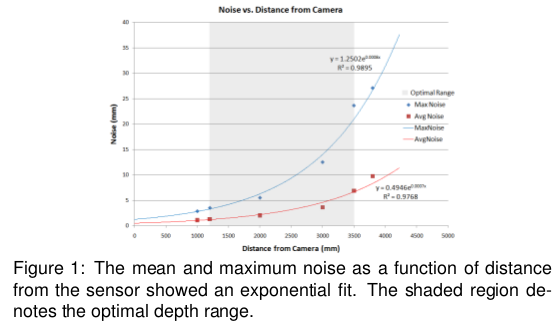
\includegraphics[scale=0.4]{./1.png}
% 1.png: 0x0 pixel, 0dpi, 0.00x0.00 cm, bb=

\newline
\newline
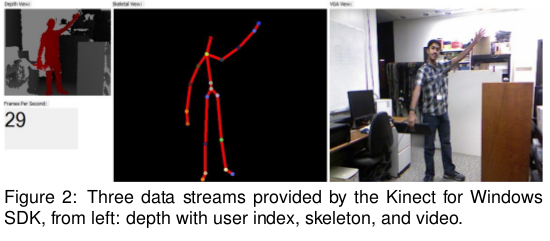
\includegraphics[scale=0.4]{./2.png}
% 1.png: 0x0 pixel, 0dpi, 0.00x0.00 cm, bb=
\newline
\newline


\subsection{Conclusion for above section}
\begin{itemize}
 \item The \strong latency is the most problematic performance characteristic. Even the best condition produces a latency of 106 ms relatively or approximately 125 ms end-t- end latency. With multiple users or a single user close to the sensor, the number of pixels being processed for tracking of human forms increased, and latency increased correspondingly. A maximum latency of 500ms was observed which is large enough to be disturbing for a user.
 \item As with any most structured light system to recover depth, Kinect's performance degrade in difficult lighting conditions. Bright fluorescent lighting can increase the noise, but still allows tracking in dark rooms. 
\end{itemize}

\end{document}         
